\chapter{Vlastní algoritmické řešení}
\label{ch:VlastniAlg}

V této kapitole se zaměříme na popis vlastního algoritmu pro detekci systolických vrcholů a odhad srdeční tepové frekvence z fotopletysmografických signálů.

Našim cílem je vytvořit jednoduchý a efektivní algoritmus, který poskytne spolehlivé výsledky pro různé typy PPG signálů.

\section{Předzpracování PPG signálu}
\label{sec:alg_preproc}

\subsection*{Načtení signálů}
\label{sec:alg_load}
% - Záznamy jsou uloženy v různých formátech, proto je nutné je převést do jednotného formátu.
%    - numpy řetězce, int, float, ... do jedné python knihovny.
% - Dovygenerujeme referenční TF z referenčních systolických vrcholů - použijeme stejný algoritmus pro výpočet ref TF jako pro výpočet TF z námi detekovaných vrcholů.

\subsection*{Rozdělení záznamů}
\label{sec:alg_split}
% - Dlouhé záznamy z CapnoBase můžeme rozdělit na kratší úseky, které budou zpracovány jednotlivě.
%   - Z osmiminutového záznamu vytvoříme 8x 1minutový úsek s 10ti procentním překryvem.

\subsection*{Filtrace}
\label{sec:alg_filter}
% - Bandpass filter - Butterworthův filtr - vlastní nastavení.
% - Na konec signál standardizujeme od -1 do 1.


\section{Detekce vrcholů}
\label{sec:alg_peaks}
% - Detekce vrcholů v 5ti sekundových oknech, které se z 50ti procent překrývají.
%   - koukáme na 5 sekund, pak posuneme o 2,5 sekundy a znovu koukáme na dalších 5 sekund.
% - standardizace signálu v okně: -1 do 1
% - nastavení prahů - min_peak_height (lokální brute force 0,3), min_peak_distance (200 bps)
% - lokal max detektor:
%       - koukne na každý vzorek a porovná ho s předchozím a následujícím vzorkem.
%       - pokud je větší než oba AND je větší než nastavené prahy, tak je to vrchol.
% - na konci jen odstraníme vrcholy, které jsou na stejném vzorku (kvůli překrývání oken), protože chceme v budoucnu pracovat i s tím, kolik jsme našli vrcholů v okně - duplikáty by nám to zkreslily.

\section{Výpočet tepové frekvence}
\label{sec:alg_hr}
% - výpočet IBI z detekovaných vrcholů + popsat matematicky IBI
% - výpočet TF z IBI: TF = 60 / median(IBI) OR TF = 60 / mean(IBI) -- my použijeme median protože počítáme, že se v minutovém úseku (nebo desetisekundovém úseku BUT PPG) může objevit nějaký výrazný artefakt, který by nám zkreslil výpočet průměru. Pro delší úseky bychom použili průměr.
% - stejný postup je i pro výpočet ref TF z referenčních vrcholů (viz. \ref{sec:alg_load}) = můžeme porovnat s naším výstupem.

\begin{figure}[t]
	\centering
	\vspace{-10mm}
	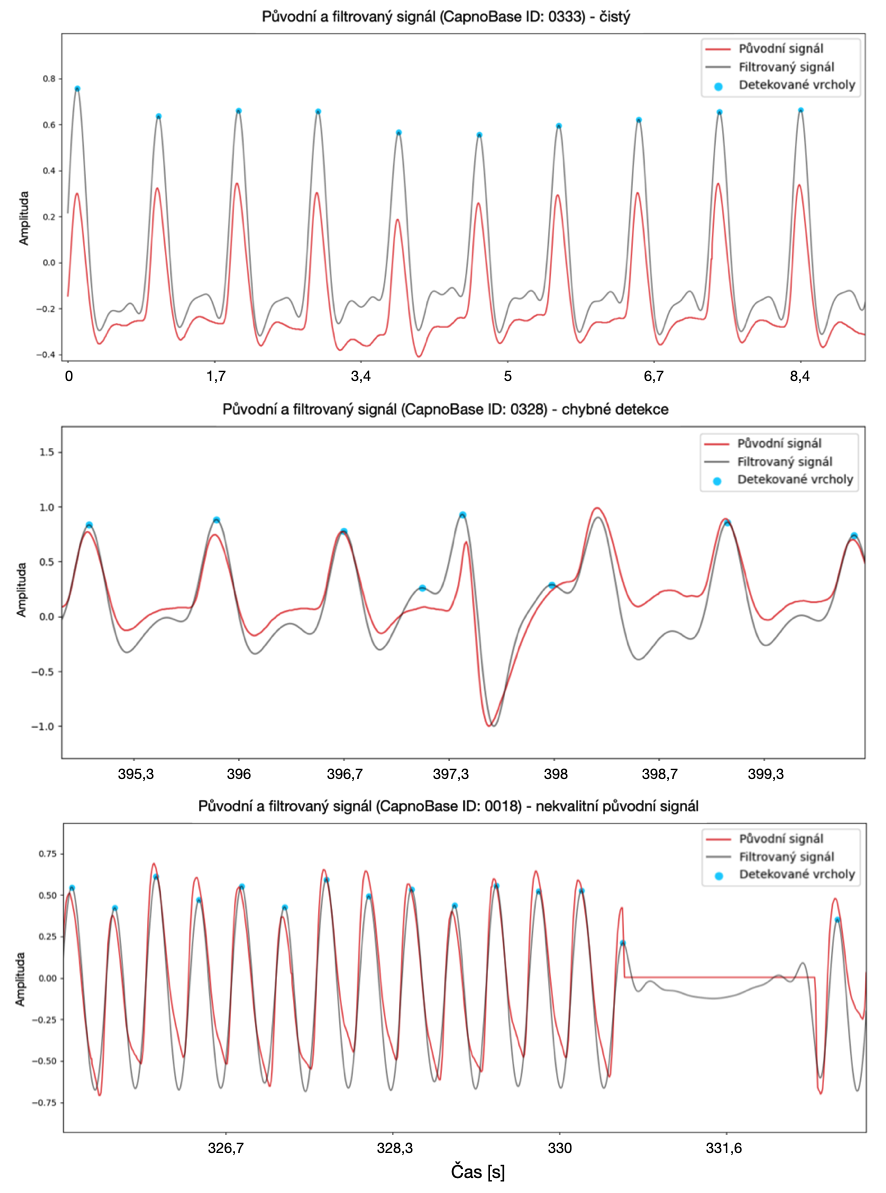
\includegraphics[width=1\textwidth]{./obrazky/MyFilterPeaks.png}
	\caption[Vlastní zpracování signálů]{...}
	\vspace{-15mm}
	\label{fig:filter-peaks}
\end{figure}